\section{Fine State Machine Realisierung}

\subsection{Realisierung von Flachen FSMs}
\begin{itemize}
  \item Steuerkonstrukt (typischerweise mit switch-case)
  \begin{itemize}
    \item prozedual oder objektorientiert
   \end{itemize}
   \item Definition und Abarbeitung einer Tabelle
  \begin{itemize}
    \item prozedual oder objektorientiert
   \end{itemize}
   \item State Pattern (Gang of Four, GoF)
  \begin{itemize}
    \item nur objektorientiert
   \end{itemize}
   \item Generisch mit Templates
  \begin{itemize}
    \item nur mit einer Sprache, die Templates unterstützt (z.B. C++)
   \end{itemize}
   \item Alle Varianten haben wie immer sowohl Vor- als auch Nachteile
   \item Bei allen Varianten sind auch Variationen vorhanden
\end{itemize}

\subsection{Realisierung mit Steuerkonstrukt (prozedural in C)}
\begin{figure}[h]
  \centering
  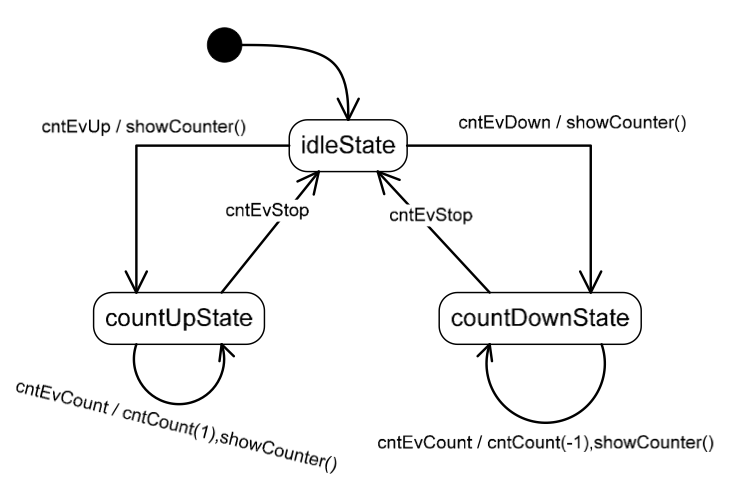
\includegraphics[scale = 0.4]{images/FSM/Up_down_counter}  
\end{figure}
\begin{itemize}
  \item Zustände (States) werden in einem eunum definiert (nicht public!)
\lstinputlisting[style=C, firstline=13, lastline=16]{snippets/Ctrl_C/counterCtrl.c}

\item Ereignisse (Events) werden in einem enum definiert (public!)
\lstinputlisting[style=C, firstline=12, lastline=16]{snippets/Ctrl_C/counterCtrl.h}

\item Die FSM wird in zwei Funktionen implementiert
\lstinputlisting[style=C, firstline=18, lastline=23]{snippets/Ctrl_C/counterCtrl.h}

\item Der aktuelle Zustand der FSM wird in einer statischen Variablen gehalten
\lstinputlisting[style=C, firstline=18, lastline=18]{snippets/Ctrl_C/counterCtrl.c}

\end{itemize}

\subsubsection{Vollständiger Code für prozedurales Steuerkonstrukt}
\lstinputlisting[style=C]{snippets/Ctrl_C/counterCtrl.h}
\lstinputlisting[style=C]{snippets/Ctrl_C/counterCtrl.c}
\lstinputlisting[style=C]{snippets/Ctrl_C/counter.h}
\lstinputlisting[style=C]{snippets/Ctrl_C/counter.c}
\lstinputlisting[style=C]{snippets/Ctrl_C/counterTest.c}

\subsection{Realisierung mit Steuerkonstrukt (Objektorientiert in
C++)}

\begin{figure}[h]
  \centering
  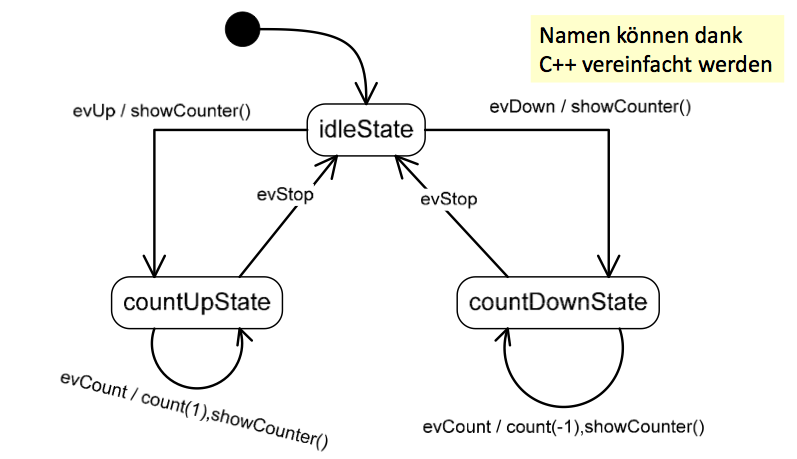
\includegraphics[scale = 0.45]{images/FSM/Up_down_counter_obj}  
\end{figure}

\begin{itemize}
  \item Logisch gesehen funktioniert die objektorientierte Variante völlig
  identisch wie die prozedurale
  \item Dank des Klassenkonstrukts kann die FSM sauber gekapselt werden
  \item Der aktuelle Zustand der FSM (currentState) wird in einem Attribut der
  Klasse gehalten
  \begin{figure}[h]
    \centering
    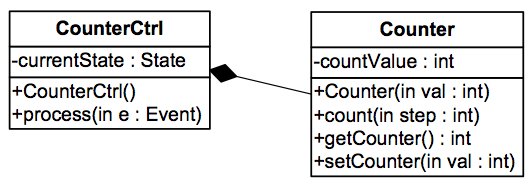
\includegraphics[scale = 0.5]{images/FSM/klasseCounter}  
  \end{figure}
  \item Mehrere Instanzen derselben FSM können einfach erstellt werden
  \item Ein Modulkürzel ist nicht notwendig, da alle Namen im Kontext von
  Klassen definiert werden
  \item Der Code wird eleganter, eine Performanceeinbusse ist nicht vorhanden
  \item States werden im \textbf{privaten-Teil} der Klasse mit einem enum
  definiert
  \lstinputlisting[style=Cpp, firstline=26, lastline=28]{snippets/Ctrl_Cpp/counterCtrl.h}

\item Events werden im \textbf{public-Teil} der klasse mit einem enum definiert
(public, weil die Events zur Schnittstelle gehören)
\lstinputlisting[style=Cpp, firstline=16, lastline=19]{snippets/Ctrl_Cpp/counterCtrl.h}

\item Die FSM wird in zwei Funktionen implementiert
\lstinputlisting[style=Cpp, firstline=20, lastline=23]{snippets/Ctrl_Cpp/counterCtrl.h}

\item \textbf{Entry-Actions} müssen überall dort hinzugefügt werden, wo in einen
neuen Zustand gewechselt wird. Üblicherweise muss die Entry-Action für einen
bestimmten Zustand bei mehreren Transitionen codiert werden.
\item \textbf{Exit-Actions} müssen überall dort hinzugefügt werden, wo ein
Zustand verlassen, d.h. in einen anderen Zustand gewechselt, wird. Üblicherweise
muss die Exit-Action für einen bestimmten Zustand bei mehreren Transitionen
codiert werden.
\end{itemize}

\subsubsection{Vollständiger Code für objektorientiertes Steuerkonstrukt}
\lstinputlisting[style=Cpp]{snippets/Ctrl_Cpp/counterCtrl.h}
\lstinputlisting[style=Cpp]{snippets/Ctrl_Cpp/counterCtrl.cpp}

\subsection{Realisierung mit Tabelle}
\begin{itemize}
  \item Die Tabelle kann sowohl prozedural als auch objektorientiert implementiert werden.
  \item Die objektorientierte Variante verwendet einzig die Datenkapselung, Vererbung und Polymorphismus werden nicht benötigt
  \item Die objektorientierte Variante kann klarer und schöner strukturiert implementiert werden. Im folgenden wird nur diese Variante gezeigt, die C-Version kann jedoch einfach davon abgeleitet werden
  \item Die ganze FSM ist in einer Tabelle gespeichert
  \item Die Aktionen sind als Funktionen implementiert, in der Tabelle steht der entsprechende Funktionspointer
  \item Die Abarbeitung der FSM erfolgt mit Hilfe einer \textit{Execution Engine}, die in der Tabelle "nachschaut", was zu tun ist
  \item Die Execution Engine ändert sich nicht, wenn die FSM geändert wird
  \item Das Testprogramm ist völlig unverändert
  \item Die Schnittstelle von CounterCtrl (public-Teil) ist ebenfalls identisch
  \item Die Klasse Counter ändert auch nicht
  \item Die \textbf{einzige Änderung} liegt im privaten Teil der
        CounterCtrl-Klasse und natürlich in deren Implementation
  \item Alle (Tansitions-)Aktionen werden als Methoden deklariert,
  \textit{Action} wird als Funktionspointer definiert. Diese Methoden müssen
  alle mit dem Funktionspointer übereinstimmen
  \lstinputlisting[style=Cpp, firstline=33, lastline=40]{snippets/Table_Simple/counterCtrl.h}

 \item Die Transition wird als klasseninterne Struktur deklariert. Sie besteht
 aus
 \begin{itemize}
   \item Aktueller Zustand
   \item Event
   \item Funktionspointer auf Aktionsmethode
   \item Nächster Zustand
 \end{itemize}
fsm() wird als statischer Array deklariert.
\lstinputlisting[style=Cpp, firstline=42, lastline=48]{snippets/Table_Simple/counterCtrl.h}

\item Tabellendefinition in CounterCtrl.cpp
\begin{figure}[h]
  \centering
  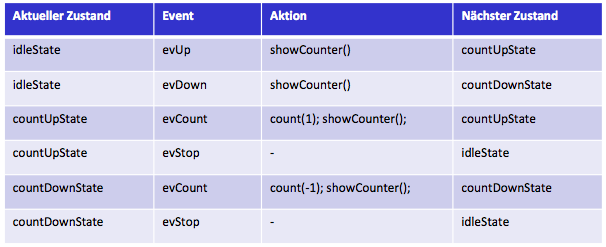
\includegraphics[scale = 0.5]{images/FSM/tabelle}  
\end{figure}
\lstinputlisting[style=Cpp, firstline=14, lastline=22]{snippets/Table_Simple/counterCtrl.cpp}

\item Aufbau einer Aktionsmethode
\lstinputlisting[style=Cpp, firstline=65, lastline=70]{snippets/Table_Simple/counterCtrl.cpp}

\item Execution Engine
\lstinputlisting[style=Cpp, firstline=30, lastline=41]{snippets/Table_Simple/counterCtrl.cpp}

\item Wenn der Zustandsübergang nicht nur durch einen Event, sondern eine
komplexe Prüfung (Event und Guard) ausgelöst wird, dann könnte der Eventeintrag
in der Tabelle durch einen weiteren Funktionspointer auf eine Checkfunktion
ersetzt werden
\lstinputlisting[style=Cpp, firstline=33, lastline=33]{snippets/Table/counterCtrl.h}
\lstinputlisting[style=Cpp, firstline=36, lastline=36]{snippets/Table/counterCtrl.h}
\lstinputlisting[style=Cpp, firstline=51, lastline=57]{snippets/Table/counterCtrl.h}
\end{itemize}

\subsubsection{Vollständiger Code für Tabellen-Realisation}
\lstinputlisting[style=Cpp]{snippets/Table/counterCtrl.h}
\lstinputlisting[style=Cpp]{snippets/Table/counterCtrl.cpp}

\subsection{Realisierung mit State Pattern}
\begin{itemize}
  \item Das Prinzip besteht aus einer abstrakten State-Basisklasse. Pro Zustand
  muss eine eigene Klasse definiert werden, die von dieser abstrakten
  Basisklasse erbt.
  \item Die Realisierung nutzt das Polymorphismus-Konzept, jede konkrete
  State-Klasse ist ein \textit{Singleton}
  \item Statt lange switch-case-if-Konstrukte wird beim State Pattern ein
  bestimmter Zustand vollständig in einer eigenen Klasse realisiert. Die Logik
  wird somit aufgeteilt.
  \item \textbf{Context} definiert die interessierenden Schnittstellen für
  Clients, unterhält eine Instanz einer konkreten Unterklasse von State, die den
  aktuellen Zustand definiert, bzw. repräsentiert
  \item \textbf{State} definiert eine schnittstelle zur FMS in Form einer
  abstrakten Klasse
  \item \textbf{ConcreteStateX Unterklassen} jede Unterklasse implementiert
  genau einen Zustand (ist Singleton)
 \begin{figure}[h]
  \centering
  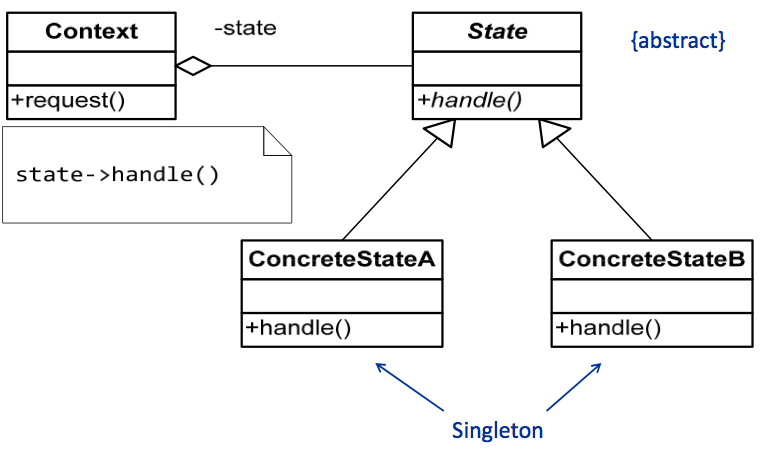
\includegraphics[scale = 0.3]{images/FSM/state_pattern}  
\end{figure}
\item Das State Pattern definiert die Zuständigkeit der state Transition nicht
\item Die Transitionen könnten in der Context-Klasse definiert werden. Der
Nachteil dieser Variante ist, dass dort zentral sehr viel Intelligenz vorhanden
sein müsste. Da diese Klasse auch den Zugriff zur Aussenwelt darstellt, sollte
sie möglichst schlank sein.
\item Die bessere Variante ist, wenn die State-Klassen auch gleich ihre
Transitionen realisieren. Diese Variante wird oft mittels friend-Deklaration
realisiert
\item Im folgenden betrachten wir eine saubere Lösung mit friend-Deklaration.
 \begin{figure}[h]
  \centering
  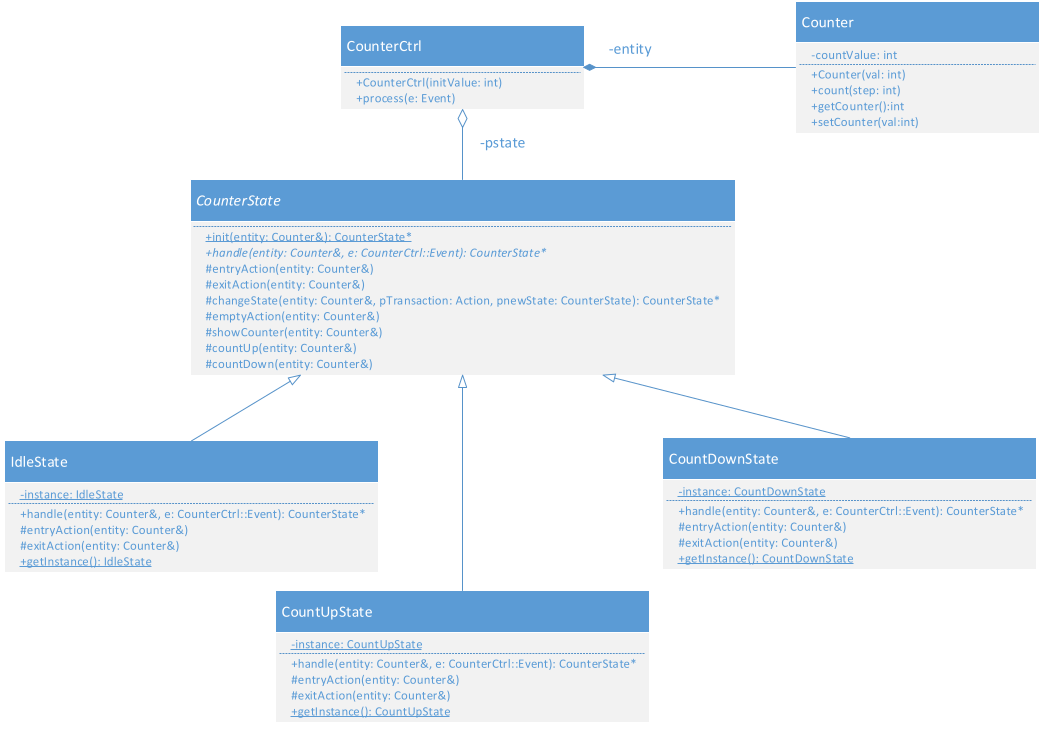
\includegraphics[height=8cm]{images/FSM/klassendiagramm}  
\end{figure}
\item counterCtrl.h : Schnittstelle zur FSM
\lstinputlisting[style=Cpp]{snippets/Pattern_Action/counterCtrl.h}

\item counterCtrl.cpp
\lstinputlisting[style=Cpp]{snippets/Pattern_Action/counterCtrl.cpp}

\item class CounterState: Interface
\lstinputlisting[style=Cpp]{snippets/Pattern_Action/counterState.h}

\item class CounterState: Implementation
\lstinputlisting[style=Cpp]{snippets/Pattern_Action/counterState.cpp}

\end{itemize}
